\documentclass{article}
\usepackage{amsmath}

%%%%%%% PACKAGES (pode ser necessário acrescentar mais, dependendo do que se pretender inserir no documento) %%%%%%%
\usepackage[utf8]{inputenc}
\usepackage[portuges,portuguese]{babel} % para podermos escrever em português
\usepackage{geometry}
\newgeometry{left=2.5cm,bottom=3cm} 
\usepackage{setspace}
\onehalfspacing 
\usepackage{subfigure}
\usepackage{hyperref}


% para que o índice possa ter o título de ``Índice'' (caso contrário fica ``Conteúdo'')
\addto\captionsportuguese{% Replace "english" with the language you use
  \renewcommand{\contentsname}%
    {Índice}%
}
\usepackage[nottoc,notlot,notlof]{tocbibind}

% para a inclusão de figuras
\usepackage{graphicx}


% para que não haja indentação no início dos parágrafos
\setlength{\parindent}{0pt} 

% para que os links apareçam como hiperligações
\usepackage{url}
\usepackage{hyperref}

\usepackage[usenames,dvipsnames]{color}    
%para introduzirmos fragmentos de script de R (ou de outra linguagem de programação)
\usepackage{listings} %para inserir excertos de codigo

\newcommand*{\authorimg}[1]{\raisebox{-.0\baselineskip}{\includegraphics[height=12pt,width=12pt,keepaspectratio,]{#1}}} %Para inserir o símbolo do R

\lstset{ 
  language=R,                     % linguagem
  basicstyle=\small\ttfamily, % tamanho das fontes usadas
  numbers=left,                   % onde colocar numeração das linhas de código
 numberstyle=\tiny\color{blue},  % estilo a usar para numeração das linhas
  stepnumber=1,                   % distância entre duas linhas numeradas (se for 1, cada linha será numerada)
  numbersep=5pt,                  % distância a que a numeração das linhas está do código
  backgroundcolor=\color{white},  % cor do background
  showspaces=false,               
  showstringspaces=false,         % sublinhar espaços em strings
  showtabs=false,                
  frame=single,                   % coloca uma moldura à volta do código
  rulecolor=\color{black},        % cor do frame
  tabsize=2,                    
  captionpos=b,                   % posição da legenda
  breaklines=true,                % line breaking automático
  breakatwhitespace=false,        
  keywordstyle=\color{RoyalBlue},      % estilo das keywords
  commentstyle=\color{YellowGreen},   % estilo dos comentários
  stringstyle=\color{ForestGreen}      % estilo das strings
} 
\begin{document}
\thispagestyle{empty}
% CAPA
\begin{flushleft}

\includegraphics[scale=0.15]{ESTB.jpg}
\end{flushleft}

\begin{center}
\Large{Instituto Politécnico de Setúb1al}
\end{center}

\begin{center}
\Large{Escola Superior de Tecnologia do Barreiro}
\end{center}

\medskip % para dar um espaço vertical


\begin{center}
\Large{\textbf{Projeto de BigData}}
\end{center}
\begin{center}
\Large{Licenciatura em Bioinformática}
\end{center}

\vspace{2cm} % espaço vertical (uma alternativa ao \medskip, que pode ser customizada para efeitos estéticos)

\begin{center}
\huge{\textbf{                                                     Visão global da taxa de suicídio 
\newline
(1985-2021)}} 
\end{center}

\vspace{7cm}
\begin{center}

\Large{Janeiro / 2023}


\large{Sérgio Pinto (202000087)}

\large{Gonçalo Rocha (202000086)}


\end{center}

% FIM DA CAPA

\newpage
\pagenumbering{roman}
%\phantomsection

% Página com o índice
\tableofcontents

\newpage
\pagenumbering{arabic}

%%%%%%% SECÇÃO "INTRODUÇÃO" %%%%%%%
\section{Introdução}\label{sec:introducao} % a label pode ser o que se quiser
Este projeto, realizado no âmbito da UC de BigData, no meu projeto, usei o dataset "Taxa de suicídio global" disponível no Kaggle, que possui 11100 linhas e 12 colunas. Este dataset contém informações sobre a taxa de suicídio global, como país, ano, gênero, idade, número de suicídios, etc. Foram utilizadas diversas bibliotecas no codigo em PySpark como seaborn, matplotlib e pyspark  Durante o projeto, os participantes desenvolveram competências no PySpark, que são utilizados para análise de dados e produção de documentos científicos, respectivamente. Isso permitiu um aumento na capacidade de trabalhar, interpretar e analisar diferentes tipos de dados.

Os resultados obtidos serão comparados e discutidos para determinar qual algoritmo de aprendizado de máquina é o melhor para prever a taxa de suicídio global. Também serão realizadas visualizações dos dados e resultados para ajudar a compreender melhor os resultados obtidos
A taxa de suicídio global é um problema de saúde pública que afeta pessoas de todas as idades e origens. A Organização Mundial da Saúde (OMS) estima que cerca de 800 000 pessoas morrem por suicídio a cada ano, o que equivale a uma morte a cada 40 segundos.
\medskip
\newline
Para a realização do trabalho foram usados os softwares nas seguintes versões: 
\medskip
\newline
•    PySpark - PyCharm Community  Edition 2022.3.1
\newline
•    Latex - TeXworks 0.6.7
\begin{figure}[h]
	\centering
	\subfigure[PyCharm]{ 
		
\includegraphics[scale=0.04]{pycharm.png}} 
	\subfigure[TeXworks]{ 
		
\includegraphics[scale=0.17]{TeXworks.png}}
	\caption{PyCharm e TeXworks}
	\label{fig:FigurasAB}
\end{figure}

\newpage
%%%%%%% SECÇÃO "DESENVOLVIMENTOS" %%%%%%%

\section{Tratamento de dados}\label{sec:Tratamento}

\subsection{Transformação dos dados}\label{sec:Transformação}

O tratamento de dados é um processo importante para garantir que os dados sejam precisos, completos e consistentes antes de serem utilizados para análise ou modelagem. Para tratar e limpar este dataset, utilizei várias ferramentas e técnicas. Primeiramente, usei o PySpark para ler e carregar os dados em um DataFrame.Isso inclui a remoção de dados duplicados, a correção de erros, a completação de dados faltantes e a normalização de dados. Além disso, foi importante verificar a qualidade dos dados, identificando e tratando valores anômalos ou outliers. Mudamos também o tipo de algumas colunas que estavam como String para Inteiro. Criamos um evaluator para calcular o indice de Silhouette de modo a obtermos o indice dos modelos. E criamos uma variável on o nosso dataset estava convertido ara Pandas, de modo a fazermos determinadas análises. Tentamos focar a seleção das features relevantes para o problema, como ano, número de suicídios, população, PIB per capita e suicidios por 100 mil pessoas. Isso foi feito para garantir que a análise e modelagem fosse baseada em dados relevantes e significativos para o problema de taxa de suicídio global. Realizamos também a divisão do dataset em treino e teste, para garantir a validade dos modelos criados.


\medskip
\section{Análise de dados}\label{sec:Analise} 
Para realizar a análise dos dados, as variáveis que mais utilizamos foram  o ano, o número de suicídios, o HDI per capita e a taxa de suicídio por 100 mil habitantes. Utilizamos também o VectorAssembler, para criar uma coluna features, que junta as colunas de interesse, e assim poder fazer previsões.

Além disso, usamos o método de avaliação Silhouette para medir a qualidadedos modelos de clusterização que aplicamos aos dados. O índice de Silhouette é um indicador da similaridade entre os objetos de um cluster em relação aos objetos de outros clusters. Quanto maior o valor de Silhouette, melhor é a qualidade do cluster.

Outra ferramenta importante foi o PySpark, que é uma biblioteca de processamento de dados distribuído para o Apache Spark. PySpark  permitiu trabalhar com grandes conjuntos de dados em paralelo, o que é essencial quando se trabalha com datasets de tamanho moderado a grande. Além disso, usamos técnicas de machine learning para analisar e modelar os dados, como o KMeans e BisectingKMeans Model. Esses algoritmos me permitiram encontrar padrões e tendências nos meus dados e fazer previsões sobre a taxa de suicídio global.

Para ilustrar as informações encontradas, usamos gráficos de dispersão e histogramas, para visualizar a relação entre as variáveis e entender melhor os dados.

\newpage
\subsection{Correlação de Pearson}
O coeficiente de correlação de Pearson mede o grau da correlação linear entre duas variáveis quantitativas. Ao contrário do coeficiente de correlação de Spearman este coeficiente requer que a relação entre as variáveis seja linear e requer que as variáveis sejam quantitativas.
\newline
Este coeficiente, assume apenas valores entre - 1 e 1. Onde 1 significa correlação negativa perfeita e +1 correlação positiva perfeita.
\bigskip
\begin{table}[h]
\begin{center}
\begin{tabular}{|r|c|c|}
\hline
&Correlação\\ \hline
Correlação entre year e suicides no & -0.028\\ \hline
Correlação entre year e population & 0.158 \\ \hline
Correlação entre year e suicides/100k pop & -0.099 \\ \hline
Correlação entre year e HDI for year & -  \\ \hline
Correlação entre year e gdp per capita   & 0.236 \\ \hline
Correlação entre suicides no e population & 0.125 \\ \hline
Correlação entre suicides no e suicides/100k pop & 0.193 \\ \hline
Correlação entre suicides no e HDI for year & - \\ \hline
Correlação entre suicides no e gdp per capita  & 0.106 \\ \hline
Correlação entre population e suicides/100k pop & -0.064 \\ \hline
Correlação entre population e HDI for year & - \\ \hline
Correlação entre population e gdp per capita  & 0.018 \\ \hline
Correlação entre suicides/100k pop e HDI for year & - \\ \hline
Correlação entre suicides/100k pop e gdp per capita  & 0.022 \\ \hline
Correlação entre HDI for year e gdp per capita  & - \\ \hline

\end{tabular}
\end{center}
\caption{Tabela dos coeficientes de correlação de Pearson das variaveis Int e Double}
\label{tab:tabela_exemplo}
\end{table}

\textbf{Análise da tabela:}
\newline
Através da tabela é possível verificar que há uma correlação fraca entre year e suicides no (-0.028), year e population (0.158) e year e suicides/100k pop (-0.099). Há uma correlação fraca positiva entre year e gdp per capita (0.236), suicides no e population (0.125), suicides no e suicides/100k pop (0.192), suicides no e gdp per capita (0.106), population e gdp per capita (0.018) e suicides/100k pop e gdp per capita (0.022).

Os valores "-" significam que não há dados disponíveis para essas combinações de variáveis, portanto, não é possível calcular a correlação.


\newpage
\subsection{Regressão linear}
A regressão linear é uma técnica de análise de dados que tenta estabelecer uma relação linear entre uma variável dependente (Y) e uma ou mais variáveis independentes (X). 

\bigskip
\begin{figure}[ht]
    \centering
   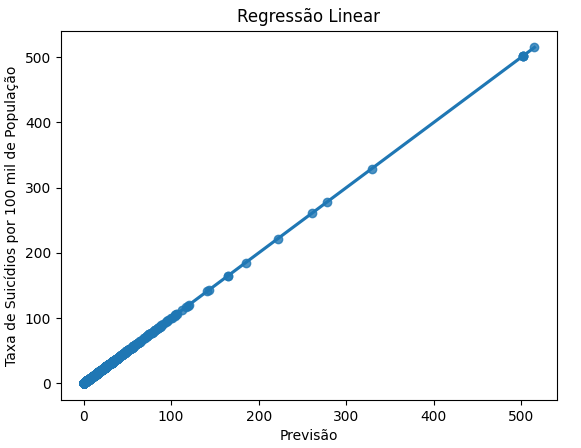
\includegraphics[scale=0.6]{regressaoL.png}
    \caption{Gráfico de Regressão Linear}
   \label{fig:RegressãoLinear}
\end{figure}
\medskip


 \textbf{Interpretação/Análise da Regressão Linear:}
\newline
 Root Mean Squared Error (RMSE): 1.33484e-09
\newline
O Root Mean Squared Error (RMSE) é uma medida de quão precisas são as previsões do modelo em relação aos dados reais. Um valor baixo de RMSE indica que o modelo está se ajustando bem aos dados. O valor de 1.33484e-09 indica que o modelo está se ajustando muito bem aos dados, pois é muito próximo de zero.Além disso, os pontos no gráfico estão todos na linha, indicando que há uma forte relação linear entre as variáveis independentes e dependentes. Isso significa que a variação nas variáveis independentes está sendo devidamente explicada pela variação na variável dependente. Isso é um indicativo de que o modelo de regressão linear é adequado para esses dados e que as previsões devem ser confiáveis.

\newpage
\subsection{Relação de suicídios entre gêneros}
O coeficiente de correlação de Pearson mede o grau da correlação linear entre duas variáveis quantitativas. Ao contrário do coeficiente de correlação de Spearman este coeficiente requer que a relação entre as variáveis seja linear e requer que as variáveis sejam quantitativas.
\newline
Este coeficiente, assume apenas valores entre - 1 e 1. Onde 1 significa correlação negativa perfeita e +1 correlação positiva perfeita.

\bigskip
\begin{figure}[ht]
    \centering
   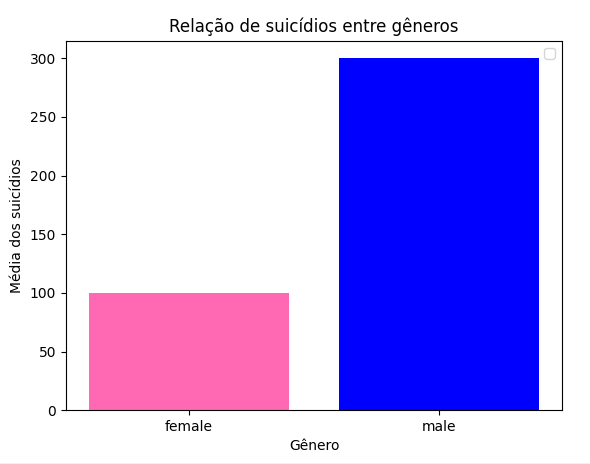
\includegraphics[scale=0.8]{graficoB.png}
    \caption{Gráfico de relação de suicídios entre gêneros}
   \label{fig:Grafsuicidgenero}
\end{figure}
 \textbf{Interpretação/Análise do gráfico:}
 \newline
O gráfico de barras mostra claramente que há uma diferença significativa entre o número de suicídios entre homens e mulheres. De acordo com o gráfico, os homens têm mais do dobro do número de suicídios em comparação com as mulheres. Isso sugere que os homens são mais propensos a cometer suicídio. Isso pode ser devido a uma variedade de fatores, como estresses sociais, econômicos e psicológicos específicos que afetam os homens de maneira diferente das mulheres.
\newpage

\subsection{Gráfico de calor}

Um gráfico de calor, também conhecido como mapa de calor, é uma representação visual de dados que utiliza cores para indicar a intensidade de um valor. Esses gráficos são usados para comparar e visualizar rapidamente grandes conjuntos de dados, como dados financeiros, climáticos ou estatísticos. Eles também são úteis para detetar tendências e padrões em dados categóricos ou numéricos. 
\newline
\bigskip
\begin{figure}[ht]
    \centering
   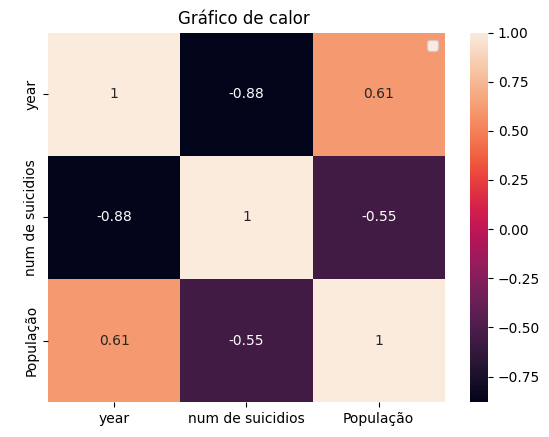
\includegraphics[scale=0.8]{mapacalor.png}
    \caption{Gráfico de calor}
   \label{fig:Graficalor}
\end{figure}
 \newline
 \textbf{Interpretação/Análise do gráfico:}
 \newline
O mapa de calor mostra a correlação entre as três variáveis: ano, número de suicídios e população. Os valores nas células indicam a força da correlação entre as variáveis, onde 1 representa uma correlação perfeita (positiva ou negativa) e 0 representa ausência de correlação.


Os primeiros três valores (1, -0.88 e 0.61) indicam que há uma forte correlação negativa entre o ano e o número de suicídios, ou seja, à medida que o ano aumenta, o número de suicídios diminui. Existe uma correlação positiva moderada entre o ano e a população, indicando que à medida que o ano aumenta, a população também aumenta.
Os próximos três valores (-0.88, 1 e -0.55) indicam que há uma forte correlação negativa entre o número de suicídios e o ano, como já mencionado anteriormente. Tendo uma correlação negativa moderada entre o número de suicídios e a população, ou seja, à medida que o número de suicídios aumenta, a população diminui.
\newpage
Por fim, os últimos três valores (0.61, -0.55 e 1) indicam que há uma correlação positiva moderada entre a população e o ano, como mencionado anteriormente. Além disso, há uma correlação negativa moderada entre a população e o número de suicídios, ou seja, à medida que a população aumenta, o número de suicídios diminui.

Concluindo que os dados do mapa de calor sugerem que há uma relação estreita entre as três variáveis.
\newpage

\subsection{Algoritmo K-means}

O algoritmo K-Means é um método de agrupamento não supervisionado que divide um conjunto de dados em k grupos (clusters) com base na similaridade entre os pontos de dados. Funciona dividindo aleatoriamente os pontos de dados em k grupos e então calcula a média de cada grupo. Os pontos de dados são então reatribuídos ao grupo cuja média é mais próxima. Este processo é repetido até que não haja mais reatribuições de pontos de dados de um grupo para outro. O K-Means é amplamente utilizado para tarefas de agrupamento.
\bigskip

\begin{figure}[ht]
    \centering
   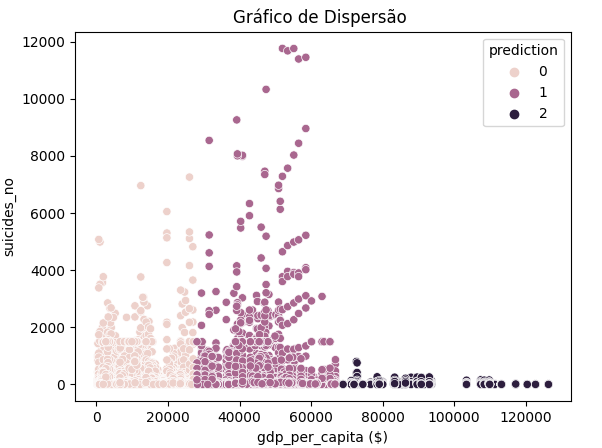
\includegraphics[scale=0.8]{grafioDK.png}
    \caption{K-means}
   \label{fig:km}
\end{figure}

 \textbf{Interpretação/Análise do gráfico:}
K-means Silhouette:0.8405099973430933
 \newline
O algoritmo K-means apresentou um valor de silhouette de 0.8405099973430933, o que indica que há uma boa separação entre os grupos formados pelo algoritmo. O gráfico de dispersão mostra que os valores na coluna "prediction" estão agrupados em três clusters diferentes, identificados pelos valores 0, 1 e 2. A partir dos dados apresentados, podemos observar que o cluster 0 está associado a um faixa de GDP per capita entre 0 a +20000, com um grande número de pontos abaixo de 2000 suicídios. Já o cluster 1 está associado a uma faixa de GDP per capita entre +20000 a +60000, com uma quantidade menor de pontos abaixo de 2000 suicídios, mas mais espalhados, alguns atingindo valores próximos a 12000 suicídios. Por fim, o cluster 2 está associado a uma faixa de GDP per capita entre +60000 a +120000, com a menor quantidade de pontos entre os três clusters e espalhados ao longo do GDP per capita. Isso sugere que existe uma relação entre o GDP per capita e o número de suicídios, com os países com GDP per capita mais elevado tendo menos suicídios.
\newpage

\subsection{Algoritmo  BisectingKMeans }

O BisectingKMeans é um algoritmo de agrupamento baseado em k-means que é usado para dividir um cluster grande em clusters menores recursivamente. Ele funciona selecionando um cluster grande, dividindo-o em dois clusters menores e, em seguida, dividindo cada um desses clusters em clusters menores. Isso é continuado até que se atinja o número desejado de clusters ou até que se alcance uma determinada medida de distância ou similaridade. Esse algoritmo é útil para lidar com grandes conjuntos de dados e clusters complexos, já que  é capaz de dividir clusters hierarquicamente e identificar subgrupos mais finos dentro de um cluster grande.
\bigskip
\begin{figure}[ht]
    \centering
   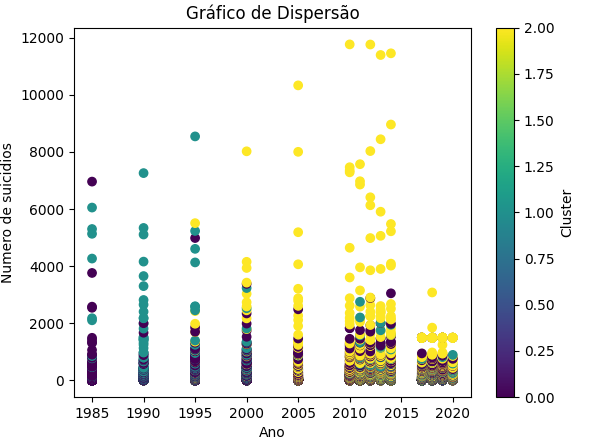
\includegraphics[scale=0.8]{garficobk.png}
    \caption{BisectingKMeans}
   \label{fig:bk}
\end{figure}
 \newline
 \textbf{a Interpretação/Análise do gráfico:}
 \newline
  BisectingKMeans silhouette: 0.6847186726707446
 \newline
De acordo com a medida de silhouette, o agrupamento obtido pelo algoritmo de BisectingKMeans tem uma qualidade média.  Logo, um valor de silhouette de 0.68 sugere que os clusters formados pelo algoritmo são razoavelmente distintos e que os pontos dentro de cada cluster são bastante similares entre si.Isto significa que o modelo de BisectingKMeans tem uma qualidade média na forma como os dados foram agrupados.
\newpage


\section{Conclusão}
Com este trabalho, podemos concluir que a  regressão linear, com um Root Mean Squared Error (RMSE) de 1.33484e-09 e todos os pontos estando na linha, podemos concluir que a regressão linear ajustou-se bem aos dados e apresentou uma boa capacidade de previsão. No entanto, é importante lembrar que a regressão linear é apenas adequada para modelar relações lineares entre as variáveis, e pode não ser a melhor escolha para modelar relações mais complexas. Quanto à regressão linear, com um Root Mean Squared Error (RMSE) de 1.33484e-09 e todos os pontos estando na linha, podemos concluir que a regressão linear ajustou-se bem aos dados e apresentou uma boa capacidade de previsão. No entanto, é importante lembrar que a regressão linear é apenas adequada para modelar relações lineares entre as variáveis, e pode não ser a melhor escolha para modelar relações mais complexas. Enquanto BisectingKMeans é um algoritmo de agrupamento de dados que é semelhante ao K-means, mas ele divide o cluster recursivamente em vez de especificar o número de clusters a priori. Quando comparado com o K-means, o BisectingKMeans pode ser menos preciso. O índice de Silhouette é uma medida comum utilizada para avaliar a qualidade de um cluster e um valor próximo de 1 indica que os dados estão bem agrupados. No caso do BisectingKMeans, o valor de 0.6847 é considerado um valor aceitável, mas é menor do que o valor obtido com o K-means (0.8405), indicando que o K-means pode ter agrupado os dados de forma mais precisa. Isso pode ser devido a que o BisectingKMeans é menos sensível aos outliers e é melhor para lidar com dados de formato diferente, mas o K-means é mais preciso. Além disso, o BisectingKMeans pode ser mais rápido do que o K-means para grandes conjuntos de dados.

\newpage
\section{Webgrafia}

\href{https://moodle.ips.pt/2223/pluginfile.php/143102/mod_resource/content/0/ML.pdf}{Disciplina:BigData}
\newline
Acedido 23 de Janeiro de 2023.
\medskip
\newline

\href{https://sparkbyexamples.com/pyspark-tutorial/l}{Spark with Python (PySpark) Tutorial For Beginners}
\newline
Acedido 16 de Janeiro de 2022.
\medskip

\end{document}
